\documentclass{standalone}
\usepackage{amsmath}
\usepackage{amssymb}
\usepackage{listings}
\usepackage{tikz}
\usepackage{xcolor}

\usetikzlibrary{calc}
\usetikzlibrary{shapes}
\definecolor{backcolour}{rgb}{0.95,0.95,0.92}
\definecolor{codepurple}{rgb}{0.58,0,0.82}

\begin{document}

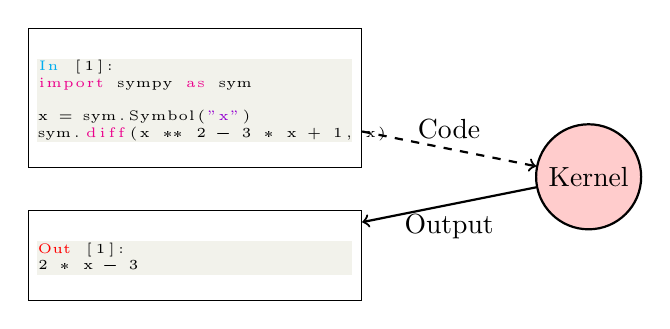
\begin{tikzpicture}
\lstset{backgroundcolor=\color{backcolour}}
\lstset{keywordstyle=\color{magenta}}
\lstset{keywordstyle=[2]\color{cyan}}
\lstset{keywordstyle=[3]\color{red}}
\lstset{stringstyle=\color{codepurple}}
\lstset{language=Python}
\lstset{morekeywords={diff, solveset}}
\lstset{keywords=[2]{In}}
\lstset{keywords=[3]{Out}}

    \node (notebook_in) [draw, text width=4cm] at (0, 0) {
\tiny
\begin{lstlisting}
In [1]:
import sympy as sym

x = sym.Symbol("x")
sym.diff(x ** 2 - 3 * x + 1, x)
\end{lstlisting}
    };

    \node (notebook_out) [draw, text width=4cm] at ($(notebook_in) + (0, -2)$) {
\tiny
\begin{lstlisting}
Out [1]:
2 * x - 3
\end{lstlisting}
    };

    \node[circle] (kernel) [draw, thick, fill=red!20] at ($(notebook_in) + (5, -1)$) {Kernel};

    \draw [->, thick, dashed] (notebook_in) -- node[above] {Code} (kernel);
    \draw [->, thick] (kernel) -- node[below] {Output} (notebook_out);

\end{tikzpicture}
\end{document}
